\section{Experiments}
Source code (C++) for both the validated integration procedure, probabilistic $\delta$-reachability, 
and the model files are available on \texttt{http://github.com/shmarovfedor/ISSRE}. 
The implementation uses the CAPD library\footnote{\url{http://capd.ii.uj.edu.pl}} for computing 
the various interval extensions required by the integration procedure. All the experiments were
carried out on a Intel Xeon E5-2690 2.90GHz system running Linux Ubuntu 12.04LTS.
\subsection{Bouncing ball}
The ball is launched from the initial point $(S_{x} = 0, S_{y} = 0)$ with initial speed 
$\upsilon_0 \sim N(20,1)$, \ie, normal distribution with mean 20 and variance 1, and angle 
to horizon $\alpha = 0.7854$. The system can be modeled as a hybrid system with one mode with 
dynamics governed by a system of ODEs: 
\[
\begin{array}{l}
S'_{x}(t) = \upsilon_0 \cos{\alpha} \\[1ex]
S'_{y}(t) = \upsilon_0 \sin{\alpha} - gt
\end{array}
\]
For simplicity we ignore the energy loss, so the speed remains constant.

The goal of the experiment is to calculate the probability of reaching the region 
$S_{x}(t) \ge 100$ within 0 and 1 jump. The results are presented in Table \ref{table:bouncing-ball}.

\begin{figure}[ht!] 
	\centering
	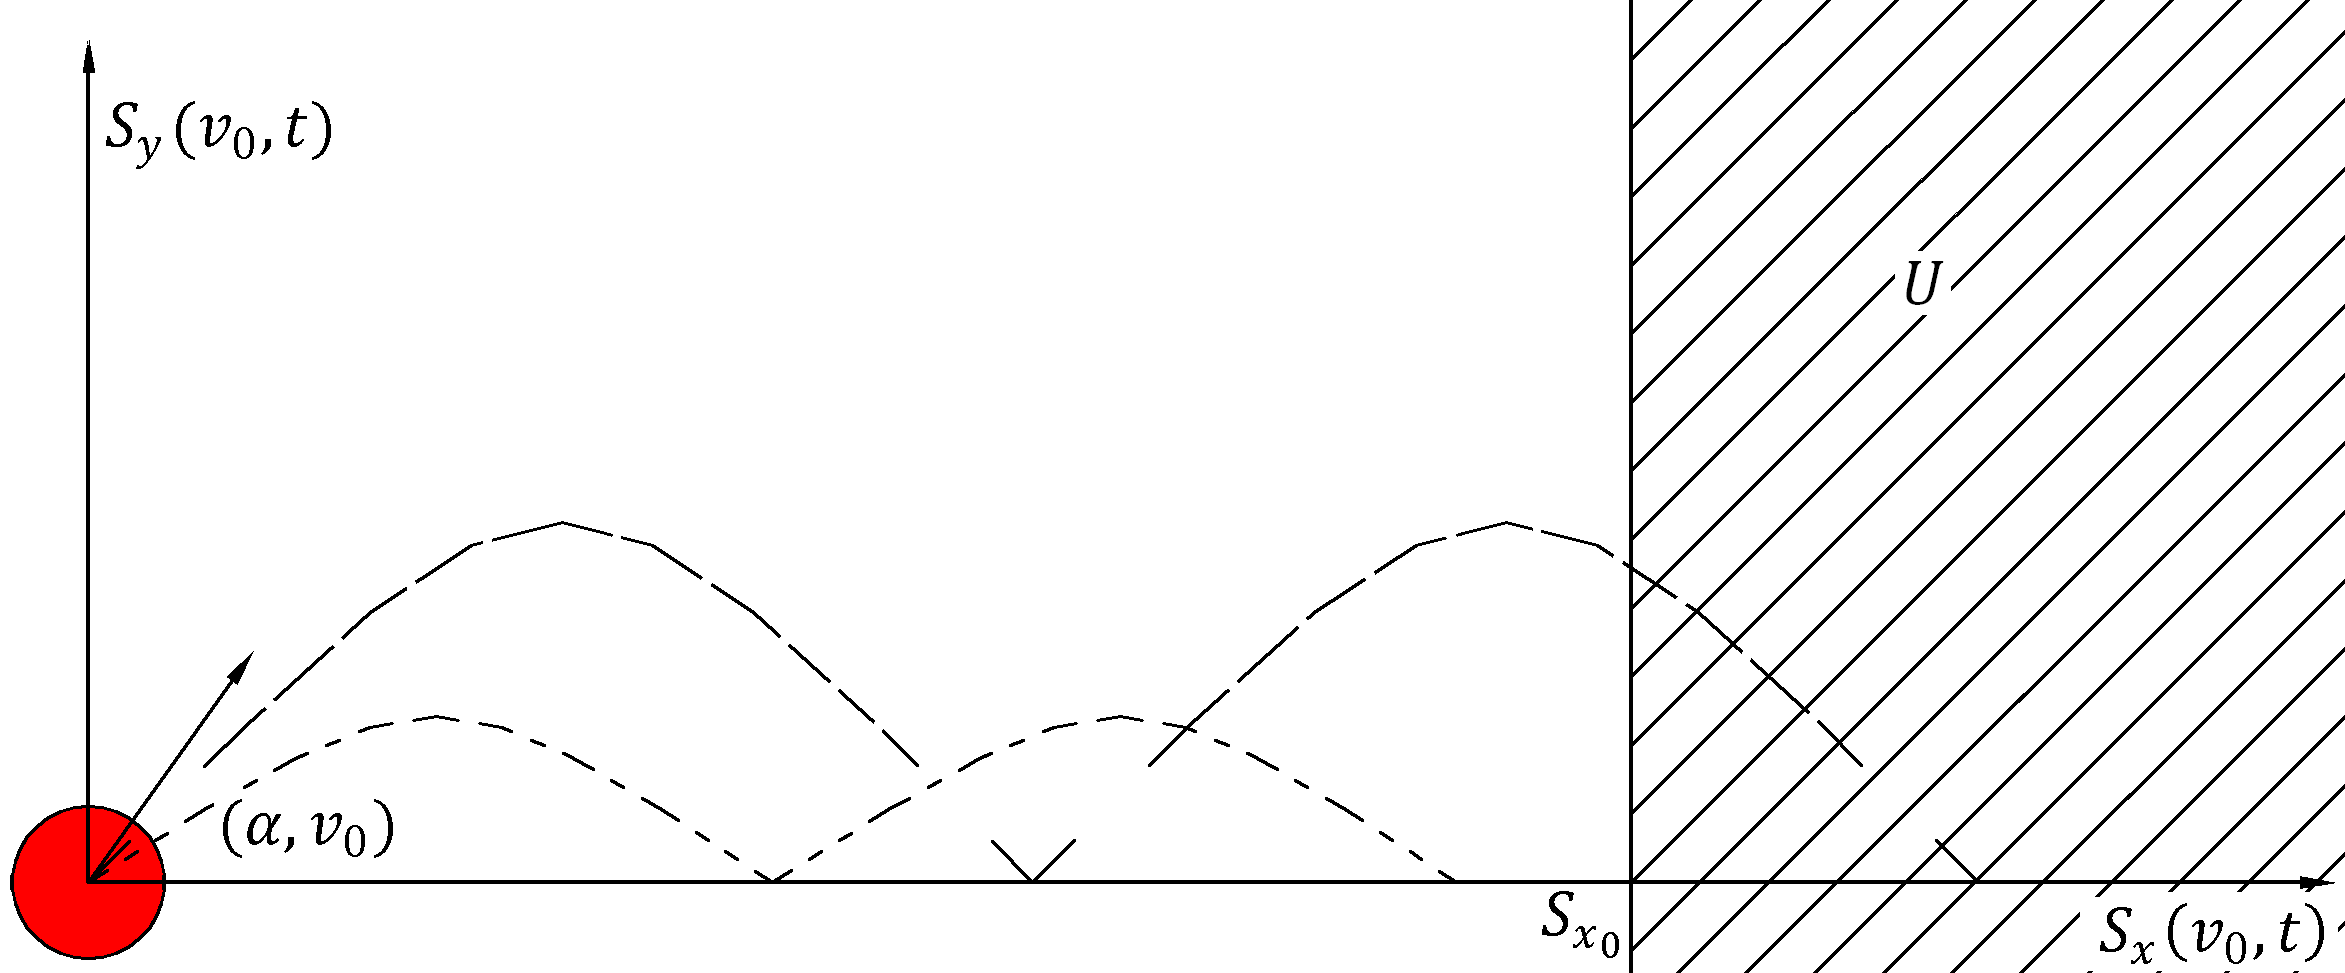
\includegraphics[width=90mm]{bouncing-ball-k-1-random-speed.png}
\end{figure}

\begin{remark}
In all experiments we use precision $\delta_1 = 10^{-12}$ for the $\delta$-complete 
procedure (dReal) and $\delta_2 = 10^{-9}$ for the integration procedure.
\end{remark}

\begin{table}[ht] 
\caption{Computing probabilistic reachability for the bouncing ball model}
\centering
\begin{tabular}{c c c c}
\hline\hline \\ [0.5ex]
\# & $k$ & Probability interval & {\em CPU}\\ [0.5ex] 

\hline \\ [0.5ex]
1 & 0 & [8.217545328383694e-05, 8.217612068446814e-05] & 82\\ [0.5ex]
2 & 1 & [0.2382375481374434, 0.2382375487609565] & 1,131\\ [0.5ex] 
\hline \\ [0.5ex]
\end{tabular} 

$k$ = number of discrete transitions, {\em CPU} = CPU time in seconds
\label{table:bouncing-ball} 
\end{table} 


\subsection{Thermostat} 
The main purpose of the system is to keep the temperature within the desired range. 
The system is modelled by two mode hybrid system \cite{DBLP:conf/hybrid/AlurCHH92} 
(Fig. \ref{fig:thermostat-2m}). The temperature is changing exponentially and it is 
decreasing in the first mode and increasing in the second mode.

The system starts in mode 1 with the initial temperature $T_{0}$ which is normally 
distributed ($\mu = 30$ and $\sigma = 1$). When the temperature drops to the minimum 
level $T_{min} = 18$, the system makes a transition to mode 2, where the temperature 
increases until it reaches a maximum level $T_{max} = 22$. Then the system makes a 
jump to mode 1 and the loop repeats again.

\begin{figure}[ht!] 
\centering
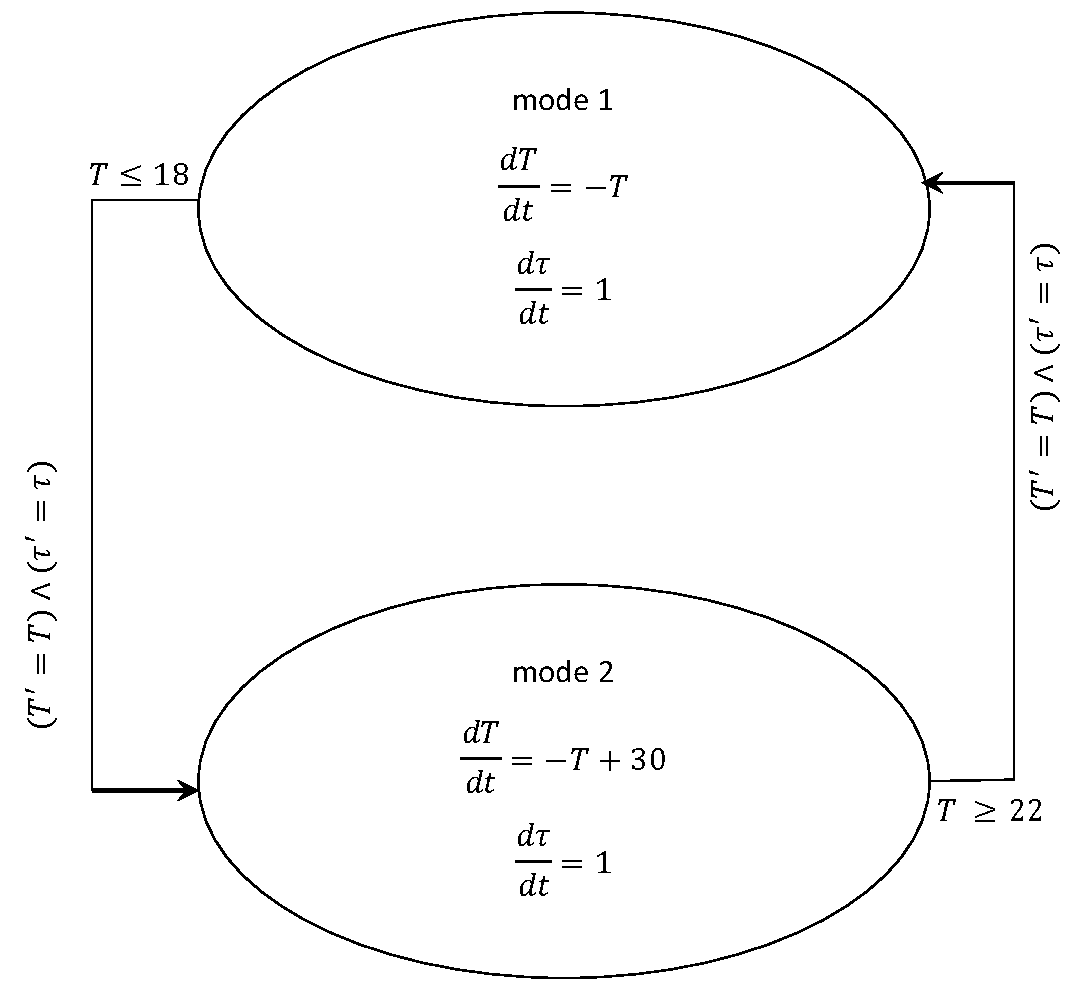
\includegraphics[width=90mm]{thermostat-2m}
\caption{A 2-mode thermostat hybrid system}
\label{fig:thermostat-2m}
\end{figure}

\begin{remark}
In the model we use function $\tau(t)$ to represent the global time, as the current
time is reset when the system makes a discrete transition.
\end{remark}

The goal of the experiment is to calculate the probability of reaching the region $T(t) \in [19.9, 20.1]$ in mode 2 at time point $\tau$. The results are presented in Table \ref{table:thermostat-2m}.

\begin{table}[ht] 
\caption{Computing probabilistic reachability of the thermostat model}
\centering
\begin{tabular}{c c c c c}
\hline\hline \\ [0.5ex]
\# & $k$ & $\tau$ & Probability interval & {\em CPU}\\ [0.5ex] 

\hline \\ [0.5ex]
1 & 1 & 0.6 & [0.006693073099383227, 0.006693073733195108] & 91\\ [0.5ex]
2 & 5 & 1.8 & [0.002635117907540255, 0.002635118445341895] & 445\\ [0.5ex] 
3 & 7 & 2.4 & [0.00160257761701815, 0.001602578290160313] & 921\\ [0.5ex] 
\hline \\ [0.5ex]
\end{tabular} 
\label{table:thermostat-2m}

$k$ = number of discrete transitions, $\tau$ = global time,
{\em CPU} = CPU time in seconds

\end{table}

We can extend the 2-mode thermostat model to a 4-mode version by adding two 
delay modes (Fig. \ref{fig:thermostat-4m}).
\begin{figure}[ht!] 
\centering
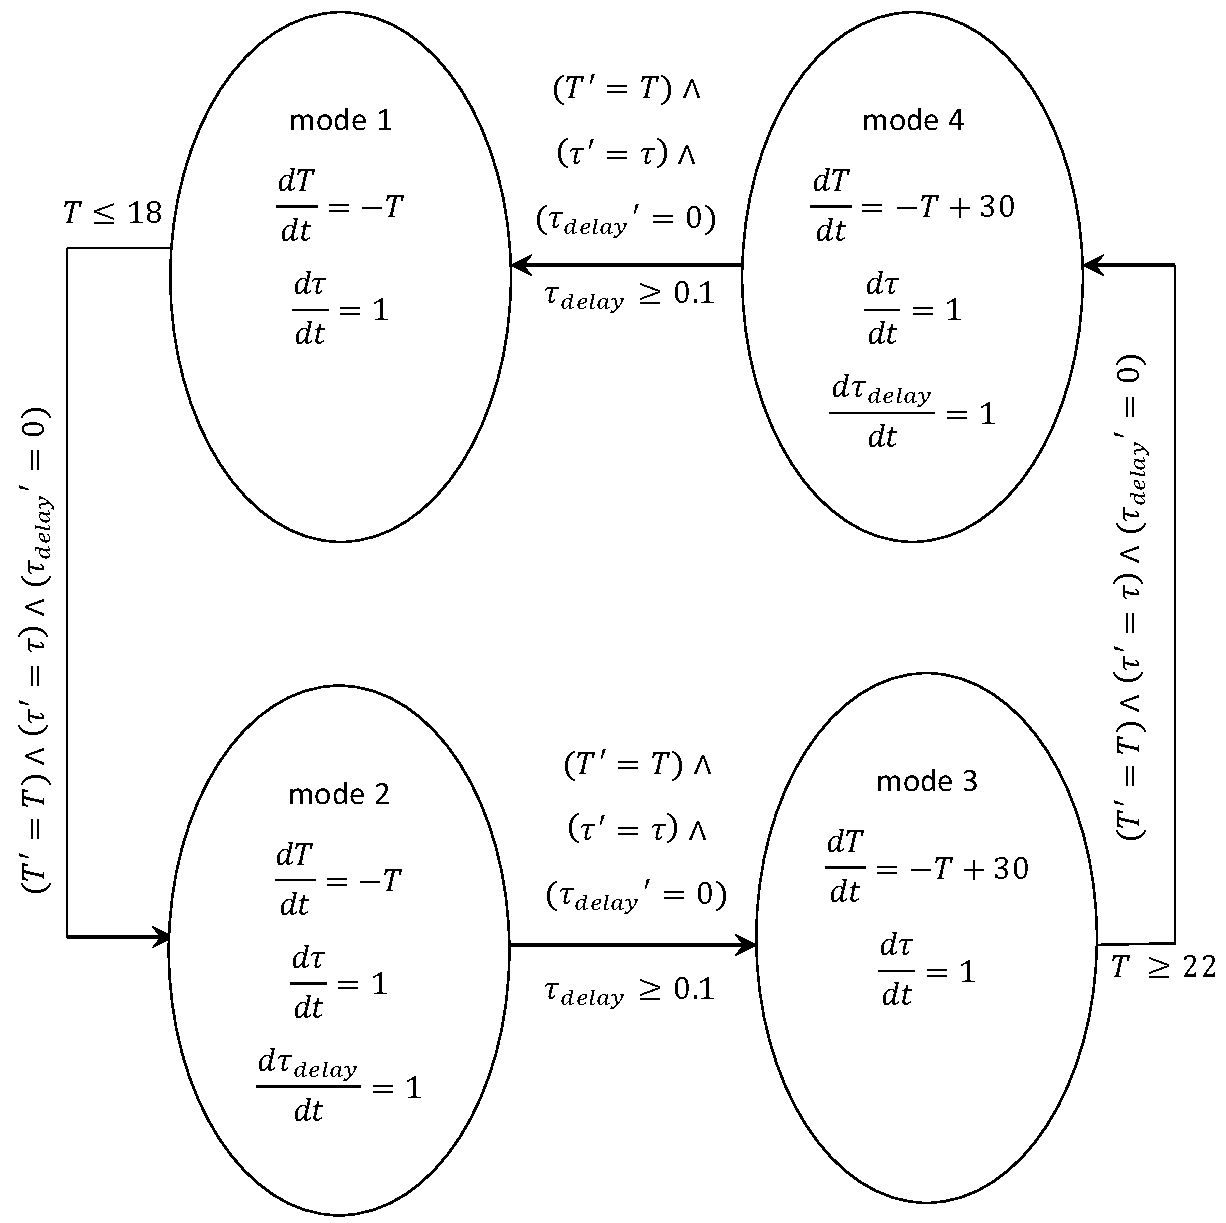
\includegraphics[width=90mm]{thermostat-4m}
\caption{A 4-mode thermostat hybrid system}
\label{fig:thermostat-4m}
\end{figure}
The initial mode of the system is mode 1. Modes 1 and 3 are equivalent to modes 1 and 2 in 
the 2-mode thermostat. Modes 2 and 4 model a delay of 0.1 seconds.
The goal of the experiment is to calculate the probability of reaching the region 
$T(t) \in [19.9, 20.1]$ in mode 3 at time point $\tau$. The results are presented in 
Table \ref{table:thermostat-4m}.

\begin{table}[ht!] 
\caption{Probabilistic reachability of the thermostat model (4 modes)}
\centering
\begin{tabular}{c c c c c}
\hline\hline \\ [0.5ex]
\# & $k$ & $\tau$ & Probability interval & {\em CPU}\\ [0.5ex] 

\hline \\ [0.5ex]
1 & 2 & 0.6 & [0, 1.707063423471755e-13] & 50\\ [0.5ex]
2 & 6 & 1.7 & [9.714528905138239e-08, 9.781433921872104e-08] & 468\\ [0.5ex] 
3 & 6 & 1.8 & [0.003995683898109569, 0.003995684421780422] & 932\\ [0.5ex] 
\hline \\ [0.5ex]
\end{tabular} 
\label{table:thermostat-4m} 

$k$ = number of discrete transitions, $\tau$ = global time,
{\em CPU} = CPU time in seconds

\end{table}

\subsection{Controlled bouncing ball}
Consider a 2-mode hybrid system (Fig. \ref{fig:controlled-bouncing-ball}) modelling a controlled 
bouncing ball \cite{ADHS09}. In mode 1, a ball of mass $m = 7$ is dropped on a platform attached 
to a stiff spring and a damper from a random height $H_{0}$, which is distributed normally 
($\mu = 9$ and $\sigma = 1$). When the ball reaches the platform ($H = 0$) the system makes a 
transition to mode 2, where the ball is reflected from the platform and it jumps back to mode 1 
when the height of the ball is greater than 0.

\begin{figure}[ht!] 
\centering
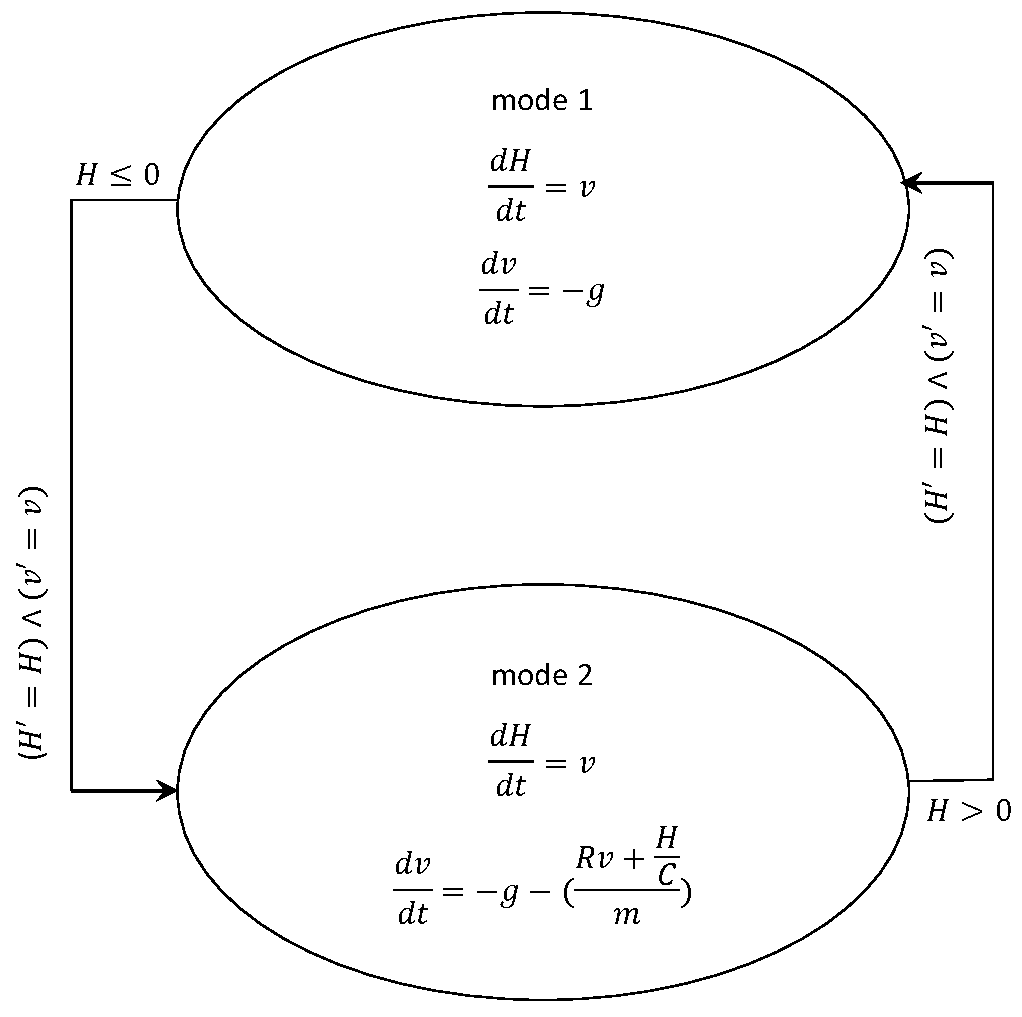
\includegraphics[width=90mm]{controlled-bouncing-ball}
\caption{A model of controlled bouncing ball with $R = 5$, $C = 0.0025$ and $g = 9.8$}
\label{fig:controlled-bouncing-ball}
\end{figure}

The goal of the experiment is to calculate the probability that the ball reaches 
the region $H >= 7$ in mode 1 after making one bounce. The results are presented 
in Table \ref{table:controlled-bouncing-ball}.

\begin{table}[ht!] 
\caption{Probabilistic reachability in the controlled bouncing ball model}
\centering
\begin{tabular}{c c c c }
\hline\hline \\ [0.5ex]
\# & $k$ & Probability interval & {\em CPU}\\ [0.5ex] 

\hline \\ [0.5ex]
1 & 2 & [0.2049030211646857, 0.2049030221625531] & 6,906\\ [0.5ex]
\hline \\ [0.5ex]
\end{tabular} 
\label{table:controlled-bouncing-ball} 

$k$ = number of discrete transitions, {\em CPU} = CPU time in seconds
\end{table}

The obtained result was validated using a simple Monte Carlo method in MATLAB. The 
time variable was discretised over the interval $[0, 5]$ in mode 1 and $[0, 0.5]$ in mode 2, 
and the system was simulated using 10,000 random samples distributed normally with mean 
$\mu = 9$ and standard deviation $\sigma = 1$. The number of samples hitting the unsafe 
region was 2,107, thereby giving a {\em probabilistic} estimate of $\frac{2107}{10,000}= 0.2107$. 
The interval returned by our validated procedure has size $0.9978674\times 10^{-9}$, and it
is {\em guaranteed} to contain the actual probability.





